\def\year{2017}\relax
%File: formatting-instruction.tex
\documentclass[letterpaper]{article} %DO NOT CHANGE THIS
\usepackage{aaai18}  %Required
\usepackage{times}  %Required
\usepackage{helvet}  %Required
\usepackage{courier}  %Required
\usepackage{url}  %Required
\usepackage{graphicx}  %Required
\frenchspacing  %Required
\setlength{\pdfpagewidth}{8.5in}  %Required
\setlength{\pdfpageheight}{11in}  %Required
%PDF Info Is Required:
  \pdfinfo{}
\setcounter{secnumdepth}{0}

\usepackage{amsmath}
\usepackage{amssymb}
\usepackage{amsthm}
\usepackage{multirow}
\usepackage{tikz}
\usepackage{comment}
\usepackage{dsfont}

\usepackage{graphicx}
\usepackage{caption}
\usepackage{subcaption}
\usepackage{listings}

\lstset{
  basicstyle=\ttfamily,
  mathescape
}


\usepackage{multicol}
\usepackage{arydshln}
\usetikzlibrary{calc,backgrounds,positioning,fit}


\newcommand{\tup}[1]{{\langle #1 \rangle}}

\newcommand{\pre}{\mathsf{pre}}     % precondition
\newcommand{\del}{\mathsf{del}}     % effect
\newcommand{\add}{\mathsf{add}}     % effect
\newcommand{\eff}{\mathsf{eff}}     % effect
\newcommand{\cond}{\mathsf{cond}}   % conditional effect
\newcommand{\true}{\mathsf{true}}   % true
\newcommand{\false}{\mathsf{false}} % false
\newcommand{\PE}{\mathrm{PE}}     % precondition
\newcommand{\strips}{\textsc{Strips}}     % precondition


\newtheorem{theorem}{Theorem}
\newtheorem{lemma}[theorem]{Lemma}
\newtheorem{definition}[theorem]{Definition}


\begin{document}

\title{Improving the Expressiveness of Planning Models with Observations of Plan Executions and Constraint Programming}

% Commented for blind submission
\author{Antonio Garrido\and Sergio Jim\'enez\\
{\small Departamento de Sistemas Inform\'aticos y Computaci\'on}\\
{\small Universitat Polit\`ecnica de Val\`encia.}\\
{\small Camino de Vera s/n. 46022 Valencia, Spain}\\
{\small \{agarridot,serjice\}@dsic.upv.es}}



\maketitle
\begin{abstract}
This paper shows that existing CSP compilations for the synthesis of temporal plans can be adapted for building temporal planning models from an initial classical planning model and a set of observations of plan executions.
\end{abstract}


\section{Introduction}
\label{sec:introduction}
{\em Automated Planning} is the model-based approach for the task of selecting actions that achieve a given set of goals. {\em Classical planning} is the vanilla model for automated planning. This planning model assumes: fully observable states, actions with deterministic and instant effects and, goals that are conditions referred only to the last reached state~\cite{geffner2013concise}.

Besides classical planning, there is a bunch of more expressive planning models that take these aspects into account to compute more detailed solutions than classical plans. One of these models is {\em temporal planning}, that relaxes the assumption of instant effects (actions can have durations, be applied in parallel and overlap) to compute plans that indicate the precise time-stamp where actions start and end~\cite{ghallab2004automated}.

Despite the potential of automated planning (state-of-the-art planners are able to compute plans with hundreds of actions in seconds time), its applicability is still limited because of the complexity of specifying correct and complete planning models. The more expressive the planning model, the more evident becomes this knowledge acquisition bottleneck. In this paper we show that existing CSP compilations for the synthesis of temporal plans can be adapted for the automatic building of temporal planning models from an initial classical planning model and a set of observations of plan executions.


\section{Background}
\label{sec:background}
This section formalizes: (1) the classical planning model we start from, (2) the {\em temporal planning} model that we aim to build (3), the kind of {\em observations} of plan executions that is given as input and (4), {\em Constraint Satisfaction Problem}, the problem solving approach we follow to address the task of building the temporal models.

\subsection{Classical Planning}
We use $F$ to denote the set of {\em fluents} (propositional variables) describing a state. A {\em literal} $l$ is a valuation of a fluent $f\in F$; i.e. either~$l=f$ or $l=\neg f$. A set of literals $L$ represents a partial assignment of values to fluents (without loss of generality, we will assume that $L$ does not contain conflicting values). We use $\mathcal{L}(F)$ to denote the set of all literal sets on $F$; i.e.~all partial assignments of values to fluents.

A {\em state} $s$ is a full assignment of values to fluents; $|s|=|F|$ with its associated time-stamp $t_s$. Explicitly including negative literals $\neg f$ in states simplifies subsequent definitions but often we will abuse of notation by defining a state $s$ only in terms of the fluents that are true in $s$, as it is common in \strips\ planning.

A classical planning action $a$ is defined as:
\begin{itemize}
\item $\pre(a)\in\mathcal{L}(F)$, the {\em preconditions} of $a$, is the set of literals that must hold for the action $a\in A$ to be applicable.
\item $\eff^+(a)\in\mathcal{L}(F)$, the {\em positive effects} of $a$, is the set of literals that are true after the application of the action $a\in A$.
\item $\eff^-(a)\in\mathcal{L}(F)$, the {\em negative effects} of $a$, is the set of literals that are false after the application of the action.
\end{itemize}
We say that an action $a\in A$ is {\em applicable} in a state $s$ iff $\pre(a)\subseteq s$. The result of applying $a$ in $s$ is the {\em successor state} denoted by $\theta(s,a)=\{s\setminus\eff^-(a))\cup\eff^+(a)\}$.

We assume that actions $a\in A$ are instantiated from given action schemas, as in PDDL. Figure~\ref{fig:flyc} shows the {\em fly} action schema from the {\em zenotravel} domain encoded in PDDL2.1~\cite{fox2003pddl2}. According to this action model an aircraft moves from one city to another consuming a single unit of fuel.

\begin{figure}[hbt!]
	\begin{scriptsize}
		\begin{verbatim}
(:action fly 
 :parameters (?a - aircraft ?c1 ?c2 - city ?l1 ?l2 - flevel)
 :precondition (and (at ?a ?c1) (fuel-level ?a ?l1)
                    (next ?l2 ?l1))
 :effect (and (not (at ?a ?c1)) (at ?a ?c2)
              (not (fuel-level ?a ?l1))
              (fuel-level ?a ?l2)))
		\end{verbatim}
	\end{scriptsize}
	\caption{PDDL1.1 encoding of the classical action model of the {\em fly} operator from the {\em zenotravel} domain.}
	\label{fig:flyc}
\end{figure}


A {\em classical planning problem} is a tuple $P=\tup{F,A,I,G}$, where $I$ is an initial state and $G\in\mathcal{L}(F)$ is a goal condition.

A {\em sequential plan} is an action sequence $\pi=\tup{a_1, \ldots, a_n}$ whose execution induces the {\em state trajectory} $s=\tup{s_0, s_1, \ldots, s_n}$ such that $s_0=I$ and, for each {\small $1\leq i\leq n$}, $a_i$ is applicable in $s_{i-1}$ and generates the successor state $s_i=\theta(s_{i-1},a_i)$. The {\em plan length} is denoted with $|\pi|=n$ . A plan $\pi$ {\em solves} $P$ iff $G\subseteq s_n$, i.e.,~if the goal condition is satisfied at the last state reached after following the application of the plan $\pi$ in the initial state $I$. A solution plan for $P$ is {\em optimal} if it has minimum length.


\subsection{Temporal Planning}
A {\em temporal planning problem} is a tuple $P=\tup{F,A,I,G}$, where $I$ is an initial state, $G\subseteq\mathcal{L}(F)$ is a goal condition, and $A$ is a set of {\em temporal actions} $a\in A$ defined as follows:
\begin{itemize}
\item $d(a)$, the action duration.
\item $\cond_s(a)\subseteq\mathcal{L}(F)$, $\cond_o(a)\subseteq\mathcal{L}(F)$ and $\cond_e(a)\subseteq\mathcal{L}(F)$, that respectively represent the {\em conditions} (literals that must hold for the action $a$ to be applicable) {\em at start}, {\em over all}, and {\em at end} of the action.

\item $\add_s(a)\subseteq\mathcal{L}(F)$ and $\add_e(a)\subseteq\mathcal{L}(F)$, that are the {\em positive effects} (fluents set to true by the application of $a$) at start and at end of the action application.
\item  $\del_s(a)\subseteq\mathcal{L}(F)$ and $\del_e(a)\subseteq\mathcal{L}(F)$, that are the {\em negative effects} (also {\em at start} and {\em at end}).
\end{itemize}
Despite temporal actions have a duration, conditions {\em at start} and {\em at end} are checked instantaneously. In the same way, {\em at start} and {\em at end} effects are instantaneously applied (effects can only happen at start or a end since continuous effects are not considered). With this regard, the semantics of a temporal action $a$ can be defined in terms of two discrete events $start_a$ and $end_a$. The duration imposes that $end_a$ must occur exactly $d(a)$ time units after $start_a$ and {\em over all} conditions of $a$ must hold in all states between $start_a$ and $end_a$. 

As an example, Figure~\ref{fig:flyt} shows the action model of the {\em fly} operator from the {\em zenotravel} domain encoded in PDDL2.1~\cite{fox2003pddl2}.

\begin{figure}[hbt!]
	\begin{scriptsize}
		\begin{verbatim}
(:durative-action fly 
 :parameters (?a - aircraft ?c1 ?c2 - city ?l1 ?l2 - flevel)
 :duration (= ?duration 180)
 :condition (and (at start (at ?a ?c1))
                 (at start (fuel-level ?a ?l1))
                 (at start (next ?l2 ?l1)))
 :effect (and (at start (not (at ?a ?c1)))
              (at end (at ?a ?c2))
              (at end (not (fuel-level ?a ?l1)))
              (at end (fuel-level ?a ?l2)))) 
		\end{verbatim}
	\end{scriptsize}
	\caption{PDDL2.1 encoding of the temporal action {\em fly} from the {\em zenotravel} domain.}
	\label{fig:flyt}
\end{figure}


A {\em temporal plan} is a set of pairs $\pi=\tup{(a_1,t_1), \ldots, (a_n,t_n)}$ such that each pair contains a temporal action $a\in A$ and its scheduled start time. Note that each $(a,t_a)\in \pi$ pair induces two discrete events, $start_a$ and $end_a$ with associated time-stamps $t$ and $t+d(a)$. If we order the $2n$ events induced from $\pi$ by their associated times, we obtain the {\em event sequence}, $E_{\pi}=\langle e_1,\ldots,e_m\rangle$, where {\small $1\leq m\leq 2n$}. Each $e_i$, {\small $1\leq i\leq m$}, is a {\em joint event} composed of one or more individual events of $\pi$ that all have the same associated time. We say that $\pi$ has {\em simultaneous events} if $m<2n$, i.e.~if at least one joint event is composed of multiple individual events. 

The {\em execution} of a temporal plan $\pi$ starting from $I$, induces the {\em state trajectory} $\tau=\tup{s_0, s_1, \ldots, s_m}$ such that $s_0=I$ and $a_i$ ({\small $1\leq i\leq m$}) is a classical planning action modeling the corresponding {\em joint event} $e_i$ and satisfying that $a_i$ is applicable in $s_{i-1}$ and that the application of $a_i$ generates the successor state $s_i=\theta(s_{i-1},a_i)$~\cite{jimenez2015temporal}. A {\em temporal plan} $\pi$ is a solution for $P$ iff the last state reached by its execution starting from $I$ satisfies that $G\subseteq s_m$.

The quality of a temporal plan is given by its {\em makespan}, i.e. the temporal duration from the the start of the first temporal action to the end of the last temporal action. Without loss of generality, we assume that the first temporal action is scheduled to start at time 0, i.e. $min_{\tup{a,t_a}\in\pi}= 0$. In this case, the makespan of a temporal plan $\pi$ is formally defined as $max_{\tup{a,t_a}\in\pi}(t_a+d(a))$


\subsection{The observation model}
In this work we assume that there is {\em partial observability} of the execution of temporal plans and that observations are {\em noiseless}, meaning that if the value of a fluent or an action is observed, then the observation is correct.

Given a {\em temporal planning problem} $P=\tup{F,A,I,G}$, and a temporal plan $\pi$ s.t. $\pi$ solves $P$ and induces the state trajectory $\tau=\tup{s_0, s_1, \ldots, s_m}$. The {\em observation} of the execution of $\pi$ on $P$ is defined as a pair $\omega=\tup{obs(\pi),obs(\tau)}$ where:
\begin{itemize}
\item $obs(\pi)$ is a sub-sequence of the pairs action-scheduled time in $\pi$.
\item $obs(\tau)$ is the same sequence of states induced by the execution of $\pi$ on $P$ but:
\begin{itemize}
\item Observed states may be partial states. The value of certain fluents may be omitted in that states, i.e.~$|s|\leq |F|$ for every $s\in obs(\tau)$.
\item Certain states may be omitted. Therefore the transitions between two con secutive observed states in $\tau$ may require the execution of more than a single action. 
\end{itemize}
\end{itemize}

\begin{definition}[$\Phi$-observation]
Given a subset of fluents $\Phi\subseteq F$ we say that $obs(\tau)$ is a $\Phi$-observation of the execution of $\pi$ on $P$ iff, for every $s\in obs(\tau)$, each observed state only contains fluents in $\Phi$.
\end{definition}


\subsection{Constraint Satisfaction Problem}
A {\em Constraint Satisfaction Problem} is defined as a triple $\tup{X,D,C}$ where:
\begin{itemize}
\item $X=\tup{x_0, \ldots, x_n}$ is a set of $n$ finite domain variables.
\item $D=\tup{D_{x_0}, \ldots, D_{x_n}}$ are the respective domains defining the set of possible values for each variable $x\in X$.
\item $C=\tup{c_0, \ldots, c_m}$ is a set of constraints bounding the possible values of the variables in $X$. Every constraint $c\in C$, is in turn a pair $c=(X_c,r_c)$ where:
\begin{itemize}
\item $X_c\subseteq X$ is a subset of $k$ variables.
\item $r_c$ is a $k$-ary relation on the corresponding subset of domains.
\end{itemize}
\end{itemize}

An {\em evaluation} of the variables is a function from a subset of variables to a particular set of values in the corresponding subset of domains. An evaluation $v$ {\em satisfies} a constraint $c=(X_c,r_c)$ if the values assigned to the variables in $X_c$ satisfy the relation $r_c$. An evaluation of $X$ is {\em consistent} if it does not violate any of the constraints in $C$. An evaluation is {\em complete} if it includes all variables. An evaluation is a {\em solution} for a given CSP $\tup{X,D,C}$ if it is both {\em consistent} and {\em complete}. 

\section{Building Temporal Planning Models}
\label{sec:learning}
Our approach for building temporal planning models from a classical planning model and observations of plan executions is to compile this task into a CSP. 

\subsection{The modeling task}
First we formalize the task of building temporal planning models from a classical planning model and a set of observations of plan executions with the pair $\Lambda=\tup{\mathcal{M},\omega}$:
\begin{itemize}
\item $\mathcal{M}$ is the set of {\bf initial action models}. This set is {\em empty}, when learning from scratch, or {\em partially specified}, when some fragments of the action models are known a priori.
\item $\omega=\tup{obs(\pi),obs(\tau)}$ is a noiseless observation of a temporal plan execution such that:
\begin{enumerate}
\item The initial state $s_0\in obs(\tau)$ is a {\em fully observed} state including positive and negative fluents, i.e.~$|s_0|=|F|$. Consequently, the corresponding set of predicates and objects that shape the fluents in $F$ are inferrable from $s_0$.
\item The header of an action model is either given by $\mathcal{M}$ or inferrable from $obs(\pi)$. In the latter case, $obs(\pi)$ must contain at least one instantiation of the respective action model header.
\end{enumerate}
\end{itemize}

A {\em solution} to a learning task $\Lambda=\tup{\mathcal{M},\omega}$ is a set of action models $\mathcal{M}'$ that is compliant with the input models $\mathcal{M}$ and the observed plan trace $\omega$.

This definition of the learning task is extensible to the more general case where the execution of several plans from the same action models are observed. In this case, $\Lambda=\tup{\mathcal{M},\Omega}$, where $\Omega=\{\omega_1,\ldots,\omega_{k}\}$ such that each $\omega\in \Omega$ is a plan trace that satisfies the previous assumptions. In this case, the {\em learned} action models $\mathcal{M}'$ have to be compliant with the input models $\mathcal{M}$ and also with every observed plan trace $\omega\in \Omega$.

\subsection{Example}
Figure~\ref{fig:plan} shows an example of a temporal plan for solving a problem from the {\em zenotravel domain}.

\begin{figure}[hbt!]
        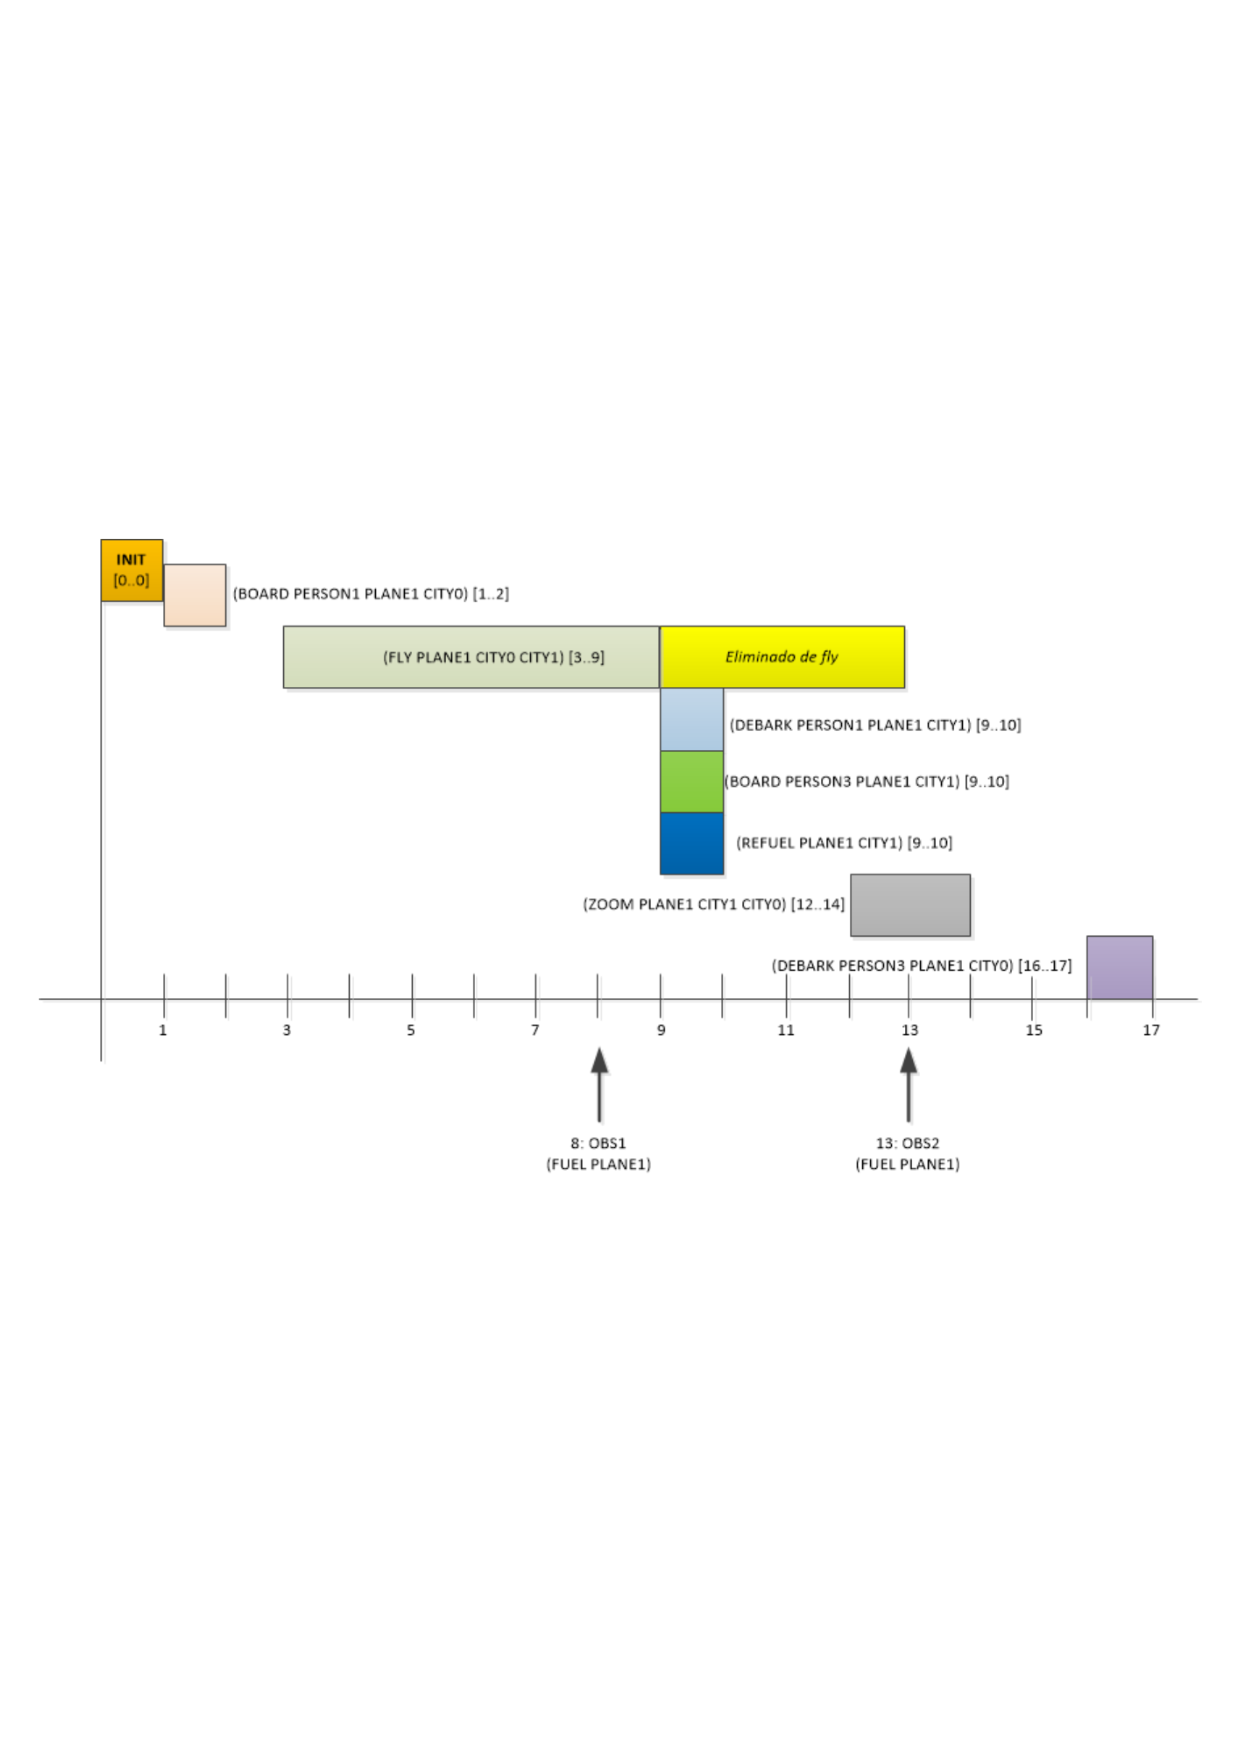
\includegraphics[width=0.5\textwidth]{plan.pdf}
	\caption{Example of a temporal plan for solving a problem from the {\em zenotravel domain}.}
	\label{fig:plan}
\end{figure}

\subsection{The compilation}
Given an observation of the execution of temporal plans $\omega$. The CSP task that is output by our compilation is built as follows.

The set of {\bf variables} $X$ comprises:
\begin{itemize}
\item For each action $a$ observed in a $\omega$:
\begin{itemize}
\item $start_a$, indicating the scheduled time-stamp for the start of the observed action $a$. The domain of this variable is $[t_a]$, i.e. a singleton given by the input observation.
\item $duration_a$ representing the action duration. The domain of this variable is $\mathds{Z}^+$.
\item $end_a$ is a derived variable, defined in $\mathds{Z}^+$, that indicates the time-stamp for the end of the observed action $a$. The value of this variable is $end_a = start_a + duration_a$. 
\item $supports_{f,a_i}$ indicates that action $a_j$ is the supporter of the fluent $f$ for action $a_i$ in the observed plan. The domain of this variable is the set of actions.
\item $preS_{f,a}$ and $preE_{f,a}$ are Boolean variables indicating whether fuent $f$ is precondition of the action $a$. The value of this variables is set by the classical planning model that is given as input.
\item $time_{f,a}$ is a variable indicating when the value of $f$ is modified as a result of applying some effects of action $a$. The domain of this variable is also $\mathds{Z}^+$.
\end{itemize}
\end{itemize}

The domains of the variables in $X$ is bound by the following set of {\bf constraints}:
\begin{itemize}
\item For each action $a$ observed in a $\omega$:
\begin{itemize}
\item $end_a = start_a + duration_a$.
\item $time_{f,a_i}!=time_{\neg f,a_j}$.
\item $time_{f,a}= start_a$ XOR $time_{f,a}= end_a$.
\item $start_a\leq preS_{f,a}\leq preE_{f,a}\leq end_a$.
\item IF $supports_{f,a_i}=a_j$ THEN:
\begin{enumerate}
\item $time_{f,a_i}\textless  preS_{f,a_j}$.
\item $time_{f,a_i}\textless  end_{a_j}$.
\item $time_{f,a_k}\textless time_{f,a_i}$ OR $time_{f,a_k}\textless time_{f,a_j}$.
\end{enumerate}
\item $(start_{a_1} = preS_{f,_{a_1}}$ AND $start_{a_n} = preS_{f,a_{a_n}})$ OR $(end_{a_1} = preS_{f,_{a_1}}$ AND $end_{a_n} = preS_{f,a_{a_n}})$. Constraints of the same kind are also defined for the variables $preE_{f,a}$ and $time_{f,a}$.
\item .
\end{itemize}
\end{itemize}

Given a solution for the CSP output by our compilation, the set of action models $\mathcal{M}'$ that solves $\Lambda=\tup{\mathcal{M},\omega}$ is computable in linear time and space. 


\subsection{Compilation properties}
\begin{lemma}
Soundness. Any solution for the CSP output by our compilation induces a set of action models $\mathcal{M}'$ that solves $\Lambda=\tup{\mathcal{M},\omega}$.
\end{lemma}

\begin{proof}[Proof sketch]
\begin{small}
\end{small}
\end{proof}

\begin{lemma}
Completeness. Any set of action models $\mathcal{M}'$ that solves $\Lambda=\tup{\mathcal{M},\omega}$ is computable solving the CSP output by our compilation.
\end{lemma}

\begin{proof}[Proof sketch]
\begin{small}
\end{small}
\end{proof}

An interesting aspect of our compilation approach is that when a {\em fully} or {\em partially specified} temporal planning model $\mathcal{M}$ is given in $\Lambda$, the compilation also serves to validate whether the observed $\omega$ follows the given model $\mathcal{M}$:

\begin{itemize}
	\item $\mathcal{M}$ is proved to be a {\em valid} action model for the given input data in $\omega$ iff a solution for the output CSP can be found.
	\item $\mathcal{M}$ is proved to be a {\em invalid} action model for the given input data $\omega$ iff the output CSP is unsolvable. This means that $\mathcal{M}$ cannot be compliant with the given observation of the plan execution.
\end{itemize}

The validation capacity of our compilation is beyond the functionality of VAL (the plan validation tool~\cite{howey2004val}) because our approach is able to address {\em model validation} of a partial (or even an empty) action model with a partially observed plan trace. On the other hand, VAL requires (1) a full plan and (2), a full action model for plan validation.

\section{Related work}
\label{sec:related}
{\em Boolean satisfiability} (SAT) is a powerful problem solving approach that has shown successful to address challenging classical planning task~\cite{kautz1999unifying,rintanen2009planning,rintanen2012planning}. Likewise {\em Constraint Satisfaction Problems} (CSP) has also been used to synthesize solution plans to numeric and temporal planning problems~\cite{do2001planning,lopez2003generalizing,vidal2006branching,garrido2009constraint}. 


\section{Evaluation}
\label{sec:evaluation}

\section{Conclusions}
\label{sec:conclusions}



\bibliographystyle{aaai}
\bibliography{tmodeling}

\end{document}
